
%%% Local Variables:
%%% mode: latex
%%% TeX-master: section01.tex
%%% End:
%%%%%%%%%%%%%%%%%%%%%%%%%%%%%%%%%%%%%%%%%%%%%%%%%%%%%%%%%%%%
 \section{现代统计图形}

\begin{frame}{科学与艺术}
  \begin{columns}
    \begin{column}{.4\textwidth}
      \begin{figure}
        \centering 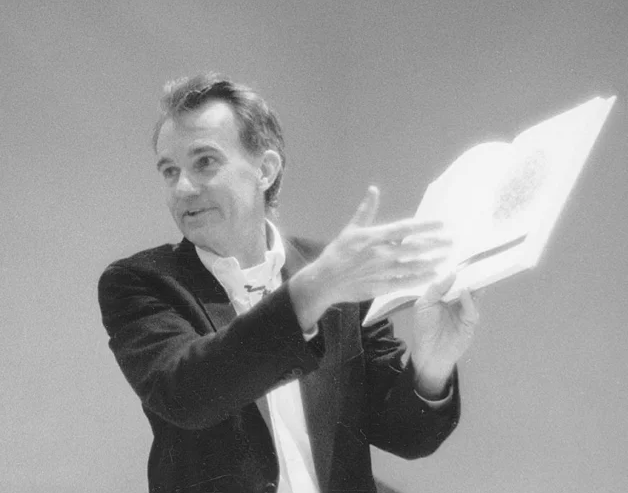
\includegraphics[width=\columnwidth]{edward_tufte.png}
        \caption{\scriptsize Edward Tufte(1942-),美国统计学家,数据可视化理论的先驱者和领军人物,人称“数据
    达芬奇”}
      \end{figure}
    \end{column}

    \begin{column}{.6\textwidth}
  \begin{ornamentblock}
    {The commonality between science and art is in trying to see profoundly - to develop strategies of seeing and showing.\\
      \rightline{\textemdash Edward Tufte}}
  \end{ornamentblock}
    \end{column}
  \end{columns}
\end{frame}

\begin{frame}{图形的价值}
  \begin{columns}
    \begin{column}{.3\textwidth}
      \begin{figure}
        \centering 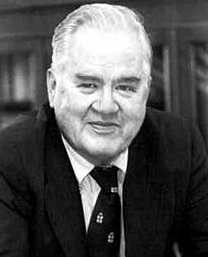
\includegraphics[width=\columnwidth]{john_tukey.png}
        \caption{\scriptsize John Tukey(1915-2000),美国著名数学家,箱线图发明者}
      \end{figure}
    \end{column}

    \begin{column}{.7\textwidth}
  \begin{ornamentblock}
    {The greatest value of a picture is when it forces us to notice what we never expected to see.\\
      \rightline{\textemdash John Tukey}}
  \end{ornamentblock}
    \end{column}
  \end{columns}
\end{frame}


%%%%%%%%%%%%%%%%
 \subsection{线图}

\begin{frame}[c]{线图(line chart)}{}
\begin{overlayarea}  {\textwidth}{\textheight}
  \only<1>{
    \begin{figure}
      \centering
      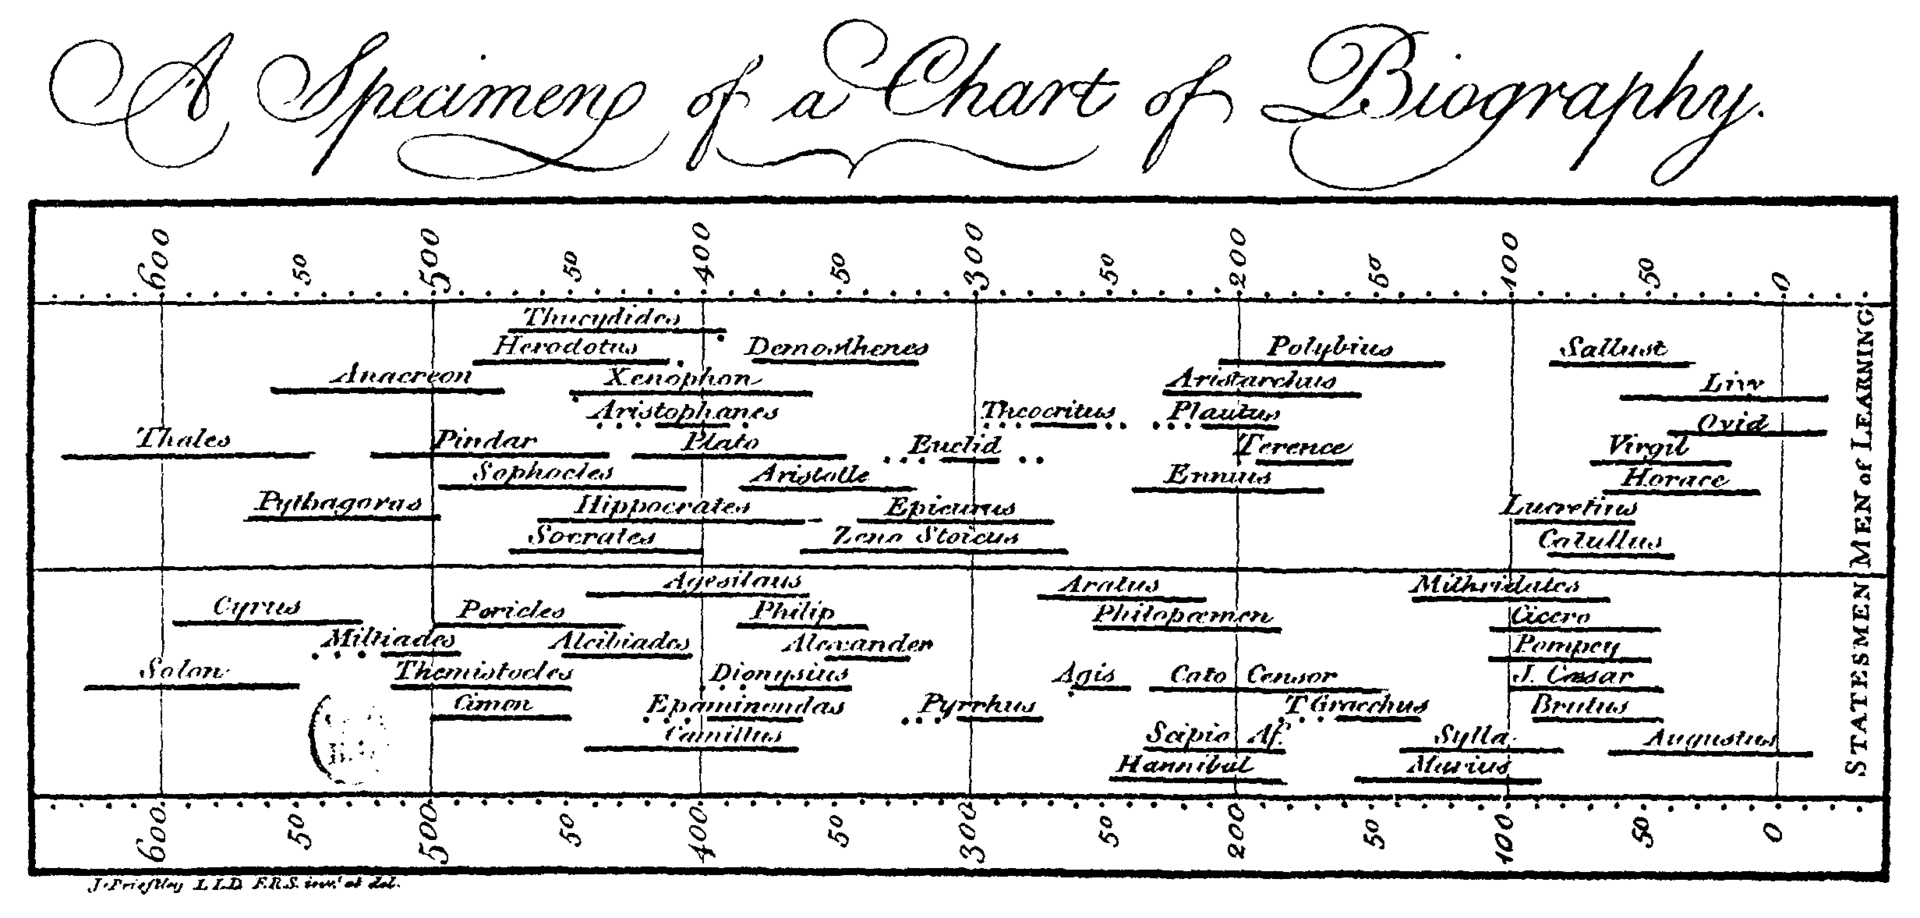
\includegraphics[width=\textwidth]{Priestley_Chart.png}
      \caption{英国化学家Joseph Priestley于1765年绘制的时间线图
        是\emphText{历史上最早的统计图形},这幅图展示了多个历史人物在历
        史长河中的跨度}
    \end{figure}} \only<2>{
    \begin{figure}
      \centering
      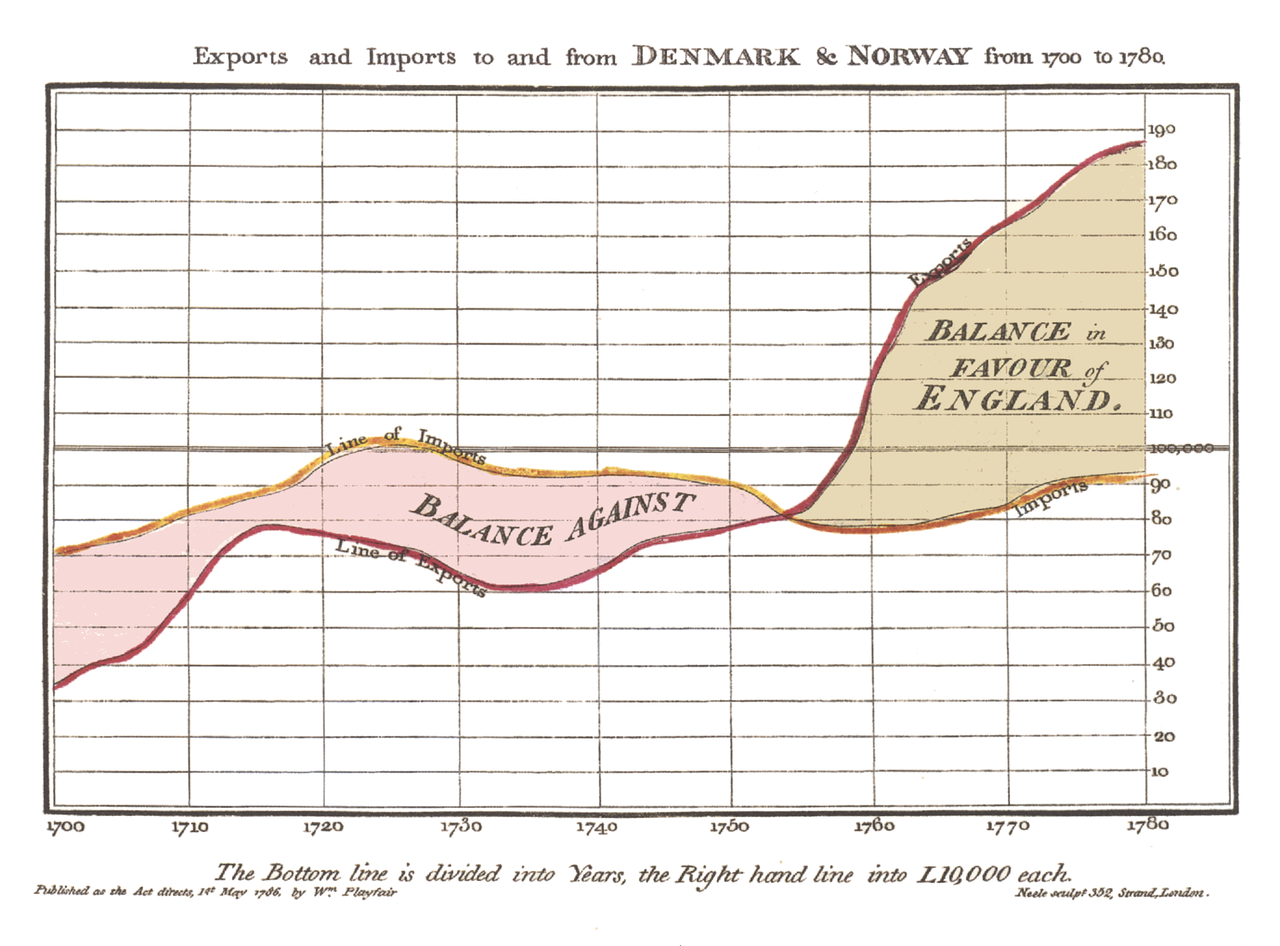
\includegraphics[width=0.75\textwidth]{Playfair_TimeSeries.png}
      \caption{苏格兰工程师和政治经济学家William Playfair于1786年在《Commercial and Political Atlas》
        一书中绘制的线图,这幅图展示了1700年至1780年间英格兰的进出口时序数据。\emphText{Playfair是历史上第一个系统使用统计图形的人,被称为“统计图形奠基人”}}
    \end{figure}}
\end{overlayarea}
\end{frame}

\subsection{柱状图}
\begin{frame}[c]{柱状图(bar chart)}{}
  \begin{figure}
    \centering
    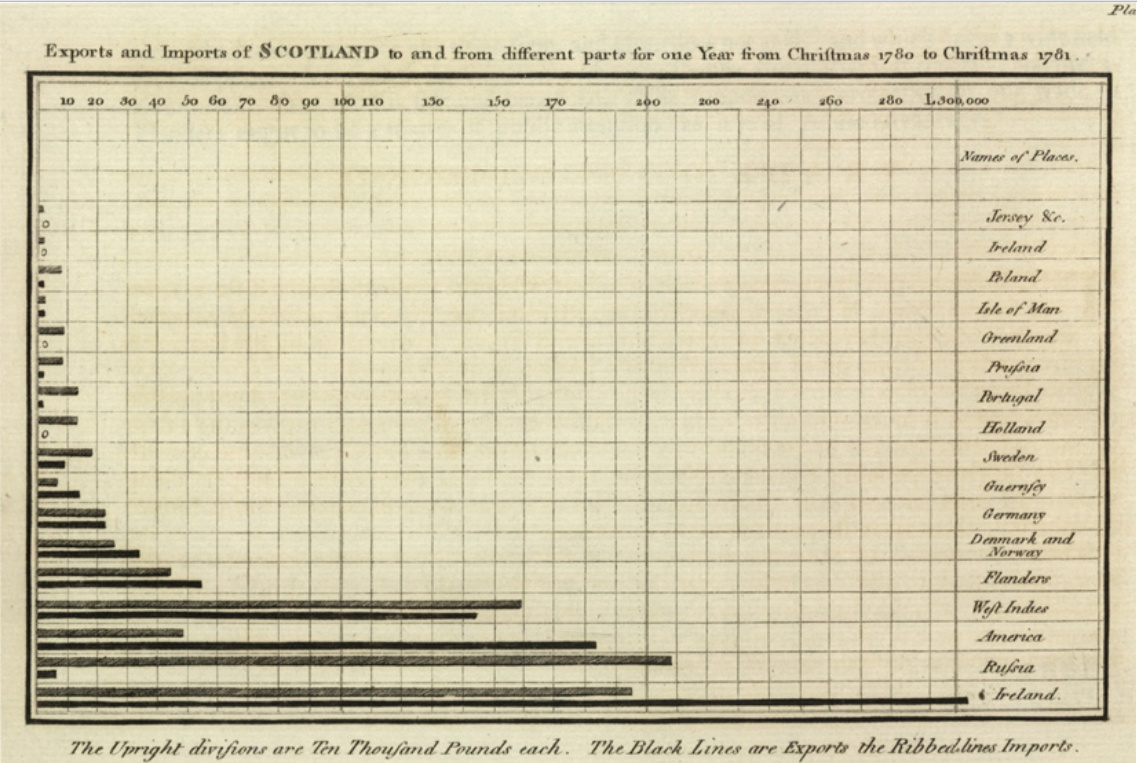
\includegraphics[width=0.8\textwidth]{Playfair_barchart.jpg}
    \caption{受到Priestley时间线图的影响,Playfair于1786年同样在
      《Commercial and Political Atlas》这本书中绘制了\emphText{历史上
        最早的柱状图},这幅图展示了不同国家的进出口数据}
  \end{figure}
\end{frame}

\subsection{饼图}

\begin{frame}[c]{饼图(pie chart)}{}
  \begin{figure}
    \begin{columns}
      \begin{column}{.6\textwidth}
        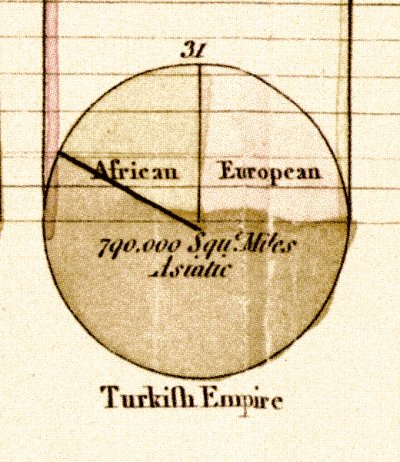
\includegraphics[width=\textwidth]{Playfair_piechart.jpg}
      \end{column}

    \begin{column}{.35\textwidth}
      \centering
      \caption{Playfair于1801年在《Statistical Breviary》这本书中绘制
        了\emphText{历史上第一幅饼图},这幅图展示了土耳其帝国在三大洲的
        国土面积分布情况}
    \end{column}
  \end{columns}
\end{figure}
\end{frame}

\subsection{主题统计地图}
\subsubsection{法国文盲率分布图}
\begin{frame}{\subsecname}{\subsubsecname}

  \begin{figure}
    \begin{columns}
      \begin{column}{.6\textwidth}
        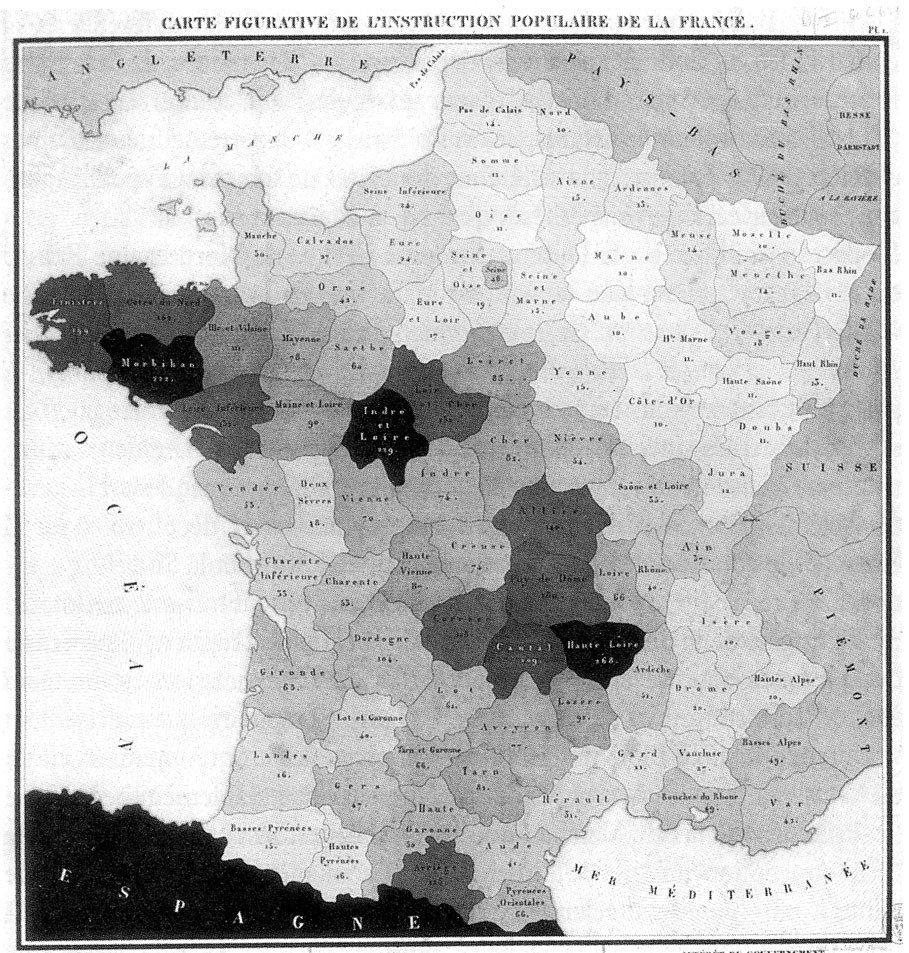
\includegraphics[width=\columnwidth]{法国文盲分布图.jpg}
      \end{column}

      \begin{column}{.35\textwidth}
        \centering
        \caption{法国文盲分布图(Charles Dupin, 1826). \\
          Charles Dupin是法国数学家,工程师,经济学家以及政客。1826年,
          他首次运用区域灰度地图的表现手段来展示法国当时的文盲率分布情
          况,\emphText{这是第一张现代形式的主题统计地图}}
      \end{column}
    \end{columns}
  \end{figure}
\end{frame}

\subsubsection{拿破仑东征图}
\begin{frame}{\subsecname}{\subsubsecname}
  \begin{figure}
    \centering 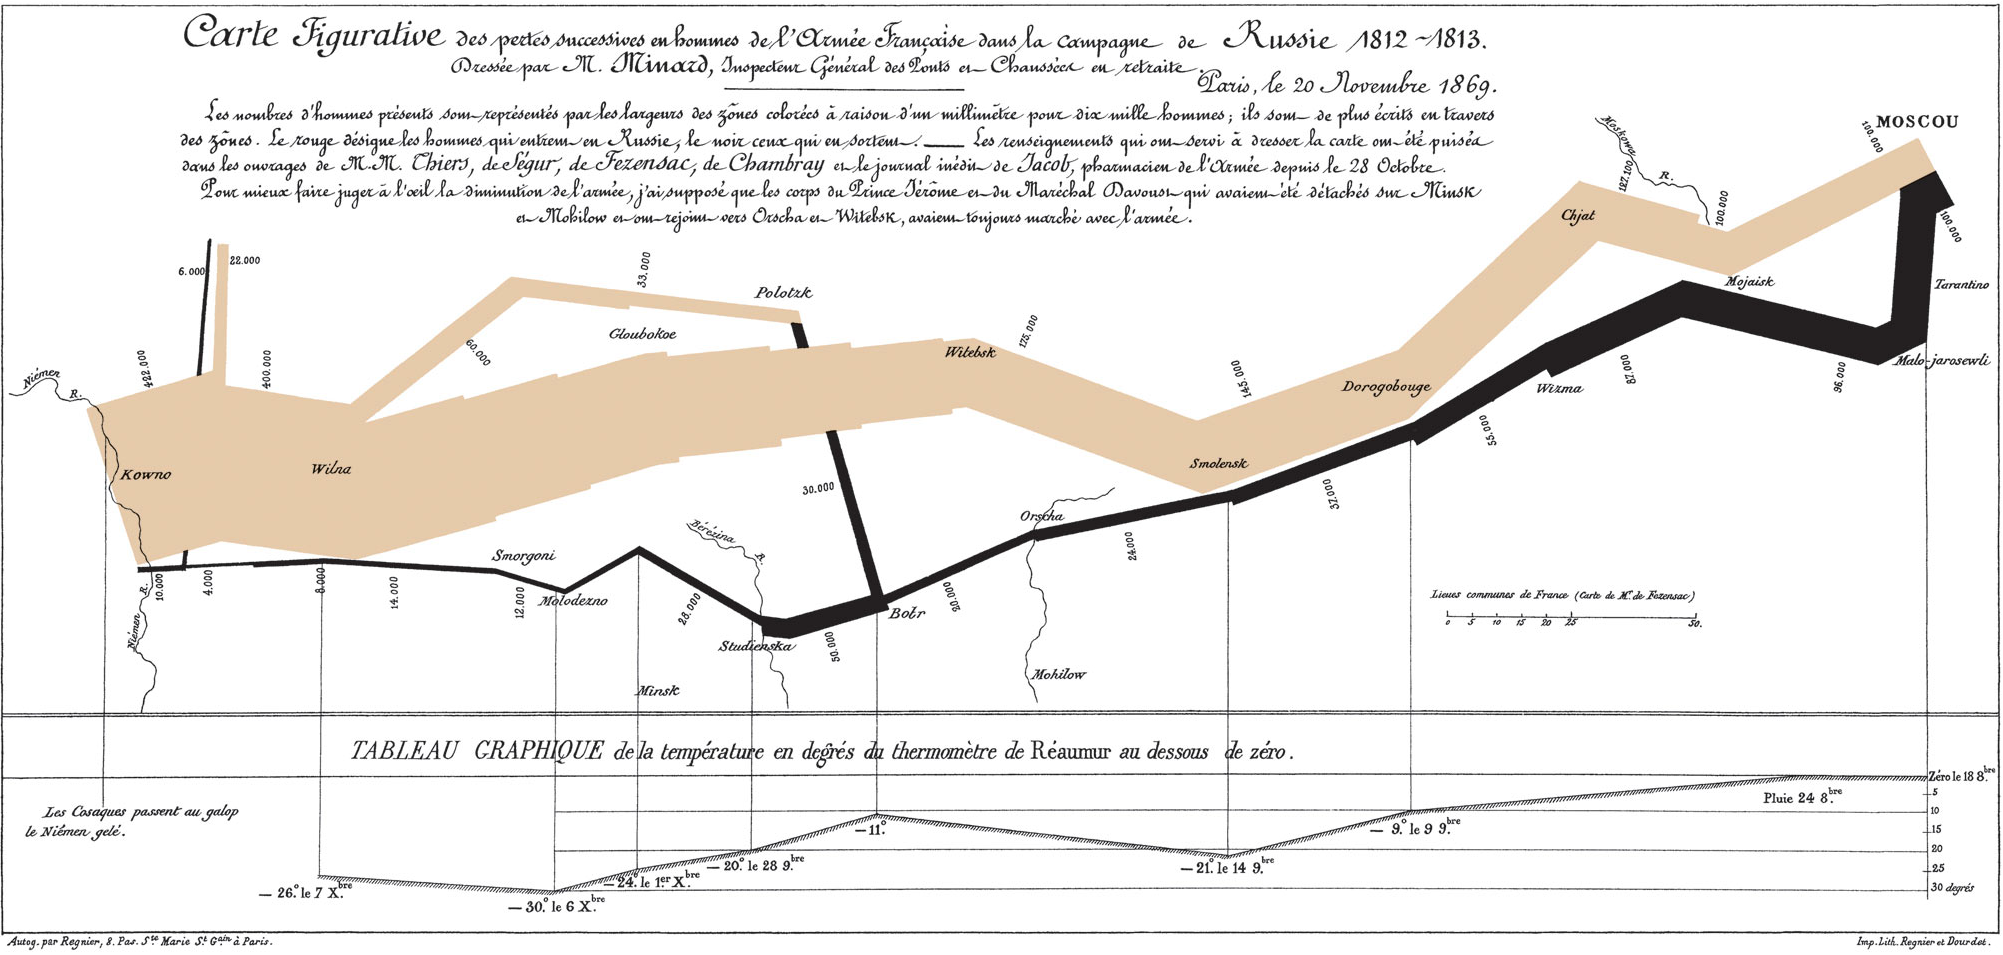
\includegraphics[width=0.8\columnwidth]{Minard.png}
    \caption{拿破仑东征图(Charles Joseph Minard, 1861). \\
      1861年,由法国工程师 Charles Joseph Minard 绘制,描述了1812年拿破
      仑东征俄罗斯的失败战役。图中同时包含了多个信息,粗细代表军队规模,
      配合日期标明了军队位置经纬度,棕色进军黑色撤退,下方折线展现气温,
      另标注了战斗的关键事件等信息。\\这幅图形在统计图形界内享有至高无上的
      地位,经常被一些统计、设计课程当作教学案例,被Edward
      Tufte誉为\emphText{“有史以来最好的统计图形”}}
  \end{figure}
  %\footnotetext[1]{Tufte是统计图形和信息可视化领域的领军人物,人称“数据达芬奇”}
\end{frame}

\subsubsection{汉尼拔远征图}
\begin{frame}{\subsecname}{\subsubsecname}
 \begin{figure}
   \centering 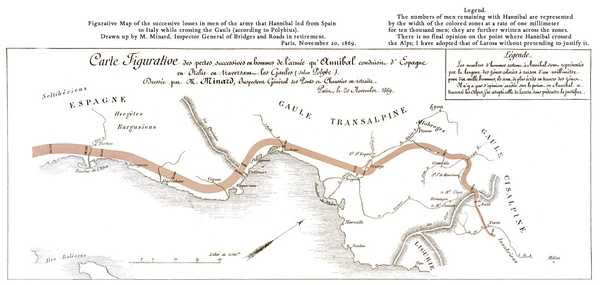
\includegraphics[width=\columnwidth]{汉尼拔远征图.jpg}
   \caption{汉尼拔远征图(Charles Joseph Minard, 1861)}
 \end{figure}
\end{frame}

\subsubsection{法国各地向巴黎输送牲畜产品的分布情况图}
\begin{frame}{\subsecname}{\subsubsecname}
  \begin{figure}
    \begin{columns}
      \begin{column}{.6\textwidth}
        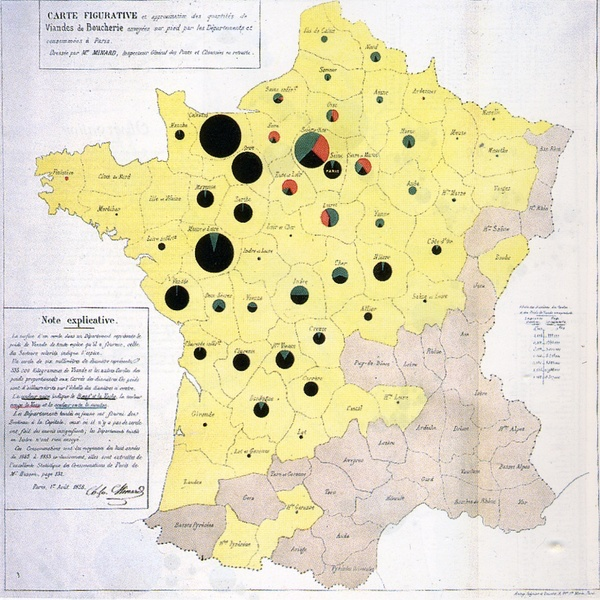
\includegraphics[width=\columnwidth]{法国各地向巴黎输送牲畜产品的分布情况图.jpg}
      \end{column}

      \begin{column}{.35\textwidth}
        \centering
        \caption{法国各地向巴黎输送牲畜产品的分布情况图(Charles Joseph Minard, 1858)\\
          此图的作者也是Joseph Minard,\emphText{经典之处在于首次将饼图融合到地图中}\\
          这位法国工程师,将一生大部分时间都贡献给了水坝,运河和桥梁的
          工程建造与教育事业,直到1851年退休,已近70岁高龄才正式开始研究数据信息图形可视化。在他最后的20年
          里,Minard在这个领域贡献了许多创新,共绘制了51幅各种形式的
          可视化图形,是那个可视化黄金时代当之无愧的大师,\emphText{被
            称为法国的“William Playfair”}}
      \end{column}
    \end{columns}
  \end{figure}
\end{frame}

\subsubsection{美国内战对欧洲棉花贸易的影响}
\begin{frame}{\subsecname}{\subsubsecname}
 \begin{figure}
   \centering 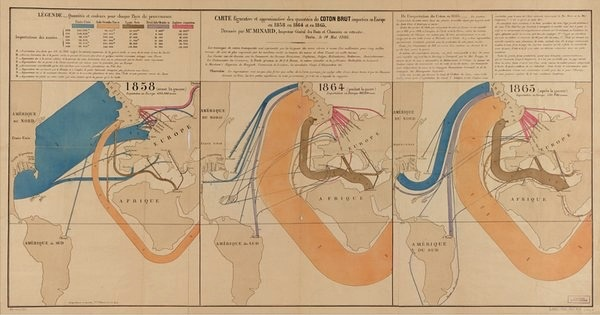
\includegraphics[width=\columnwidth]{美国内战对欧洲棉花贸易的影响.jpg}
   \caption{美国内战对欧洲棉花贸易的影响(Charles Joseph Minard, 1865)}
 \end{figure}
\end{frame}

\subsubsection{法国红酒出口情况}
\begin{frame}{\subsecname}{}
 \begin{figure}
   \centering 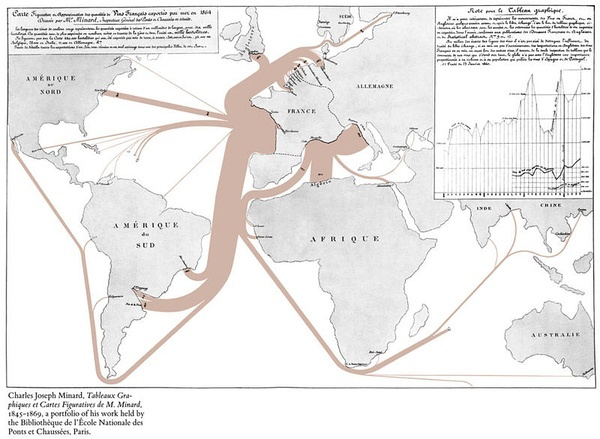
\includegraphics[width=0.8\columnwidth]{法国红酒出口情况.jpg}
   \caption{美国内战对欧洲棉花贸易的影响法国红酒出口情况(Charles
     Joseph Minard, 1864)}
 \end{figure}
\end{frame}

\subsubsection{地铁路线图}
\begin{frame}{\subsecname}{\subsubsecname}
  \begin{figure}\centering
    \subfloat[1908年版]
    {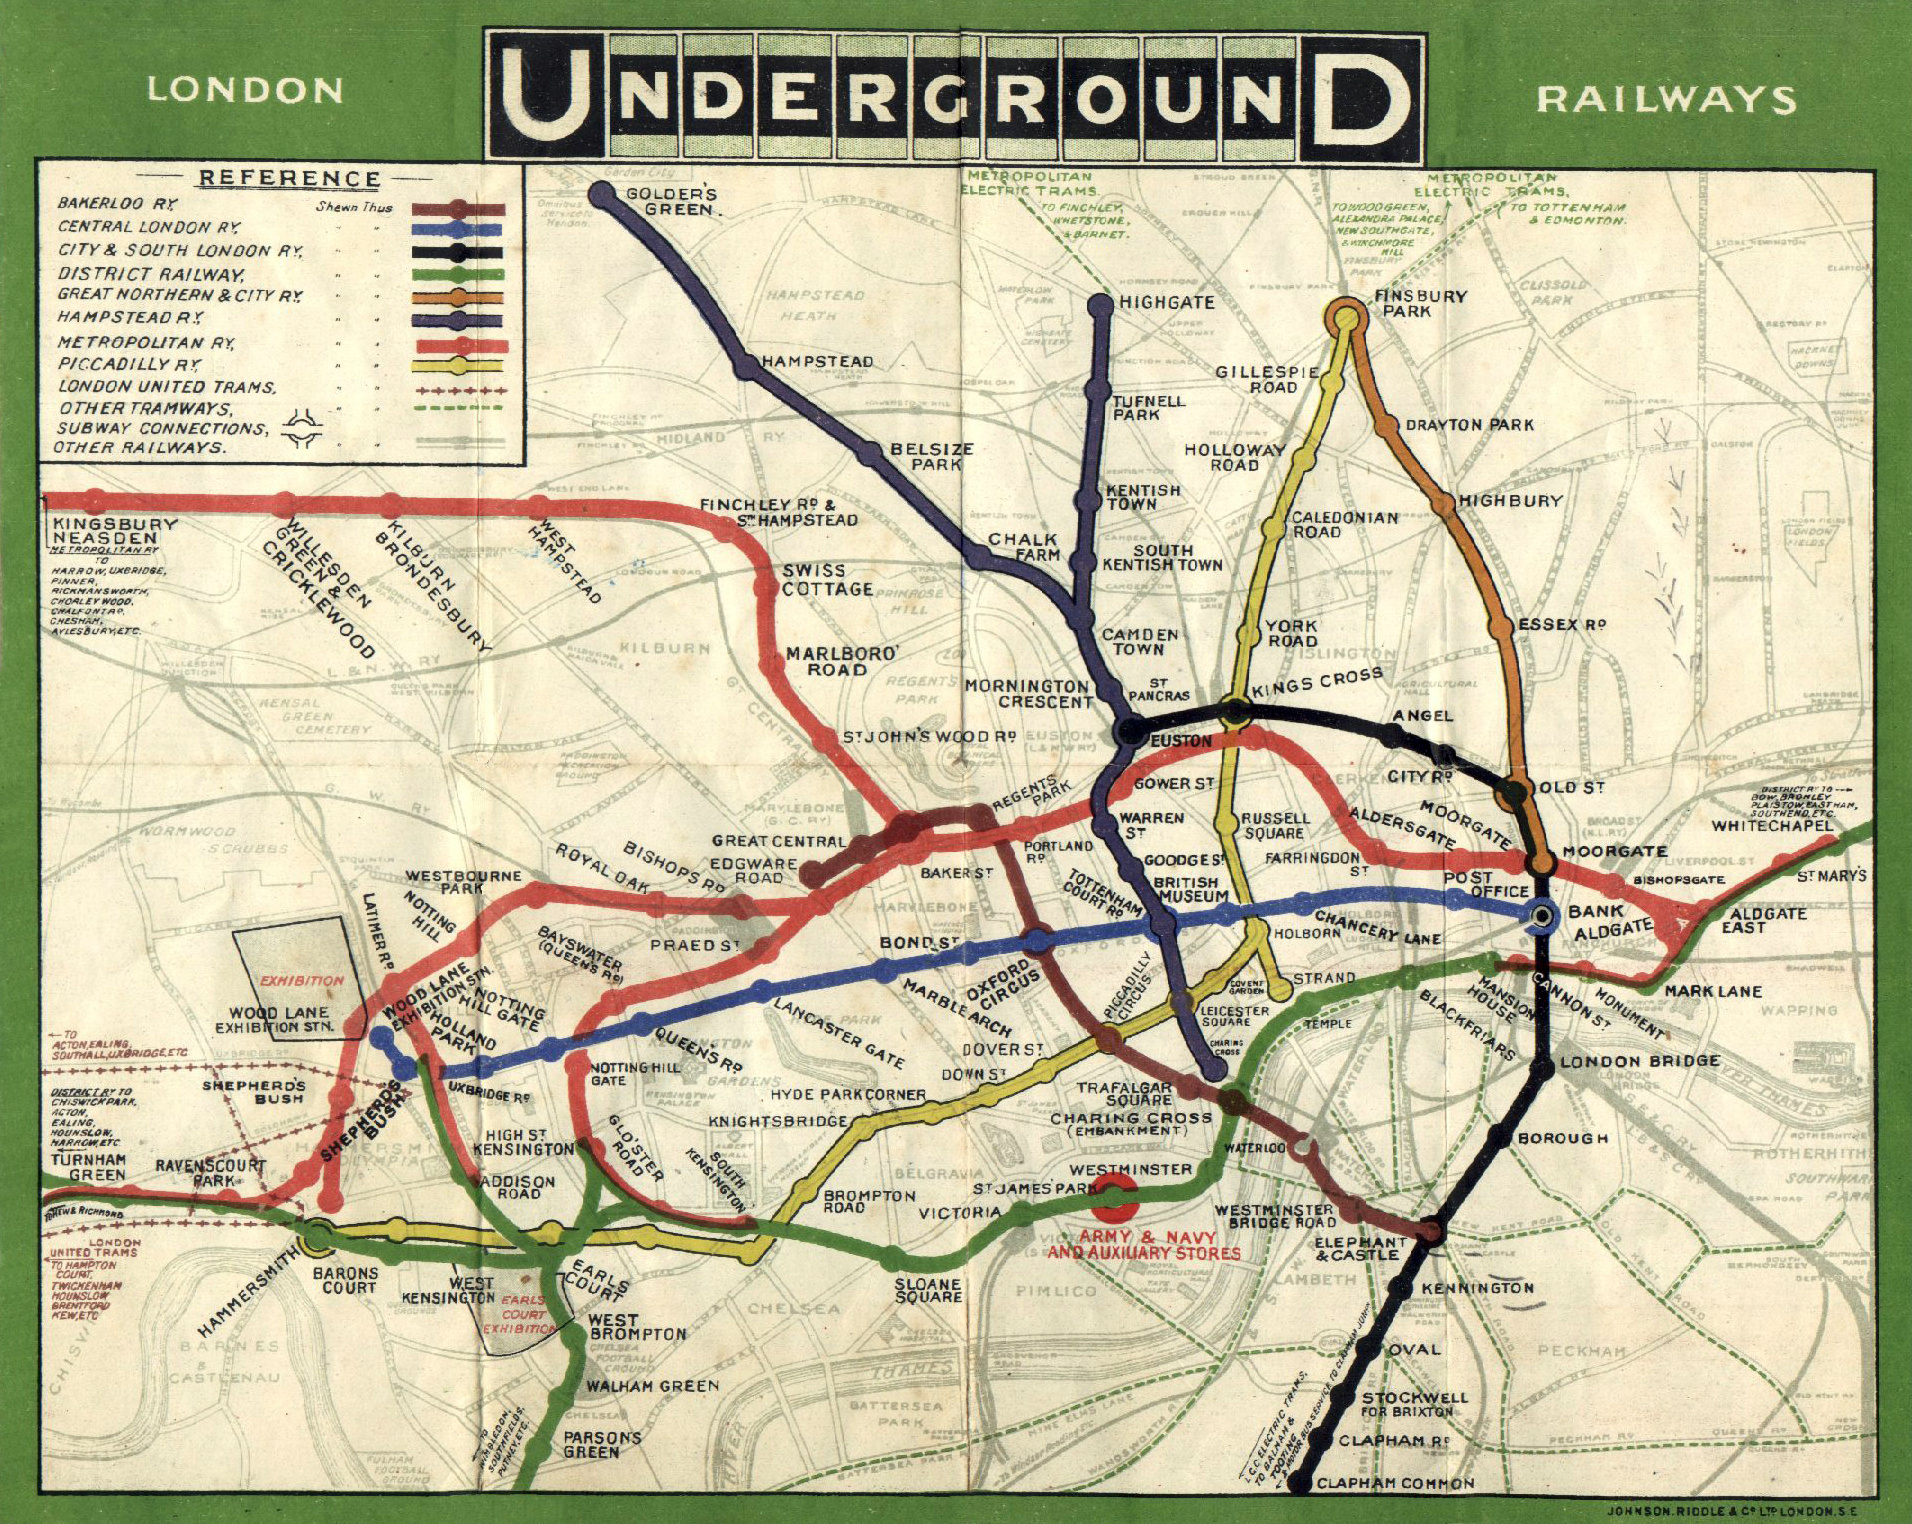
\includegraphics[height=0.4\textheight]{1908年伦敦地铁路线图.jpg}}\vspace{0.5pt} 
    \subfloat[1933年版]
    {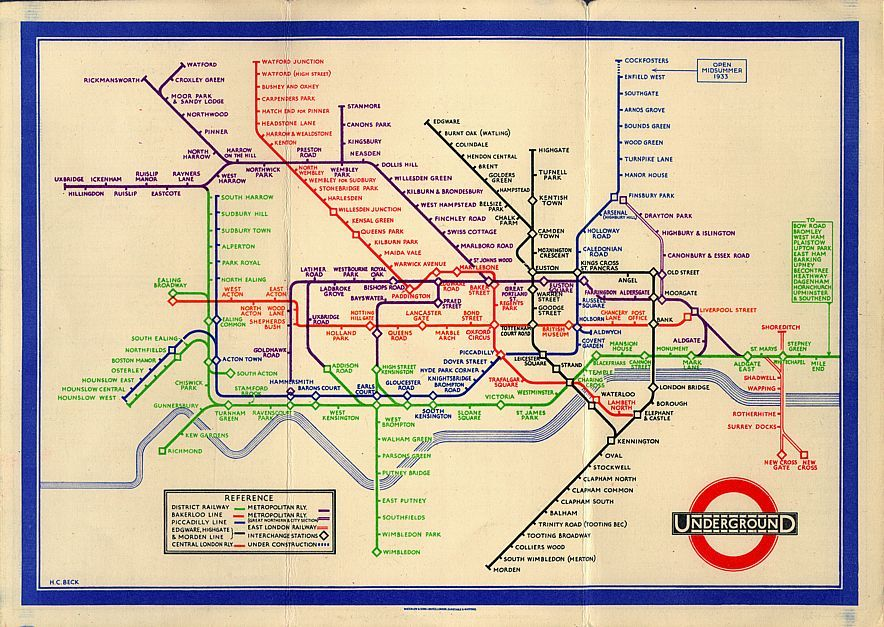
\includegraphics[height=0.4\textheight]{1931年贝克设计的伦敦地铁路线图.jpg}}
    \caption{道路网络形状更新在最早的地图中都是按照实地比例进行绘制的,
      比如左图的1908版伦敦地铁线路图。1931年,英国技术制图员Harry
      Beck在替伦敦地铁的讯号室绘制电路图时受到启发,设计出了经典
      的1933年版路线图(右图)}
  \end{figure} 
\end{frame}

\subsubsection{变形地图(cartogram)}
\begin{frame}{\subsecname}{\subsubsecname}
  \begin{figure}\centering
    \subfloat[普通色块地图表达]
    {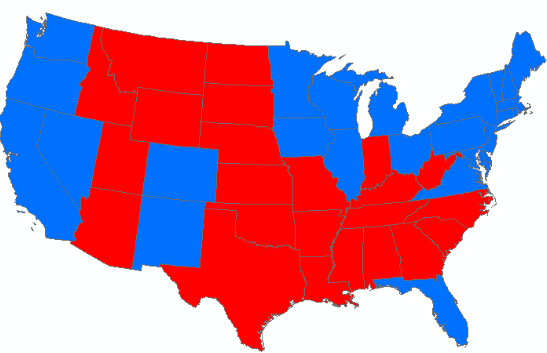
\includegraphics[width=0.45\columnwidth]{cartogram1.png}}\vspace{0.5pt}
    \subfloat[变形地图表达]
    {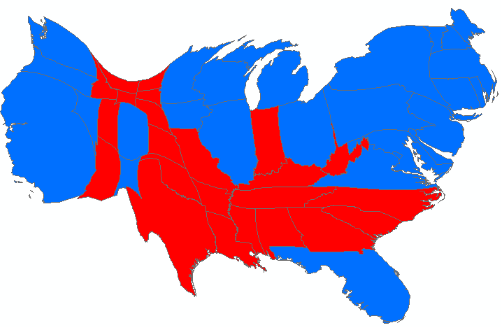
\includegraphics[width=0.45\columnwidth]{cartogram2.png}}
    \caption{变形地图的历史可以追溯到1868年,\emphText{其作用是用夸张的地图变形来表达真实的数量关系}\\上面左图是2012年
      美国大选的结果,从普通色块图上看似乎是红色代表的罗姆尼获胜,但其实获胜的是蓝色代表的奥巴马;右图是根据选票
      数量进行变形处理后的地图,可以很清楚看到蓝色多于红色,这才是真实数量的正确表达!}
  \end{figure}
\end{frame}

\subsection{统计图形的应用}
\subsubsection{南丁格尔玫瑰图}
\begin{frame}{\subsecname}{\subsubsecname}
 \begin{figure}
   \centering
   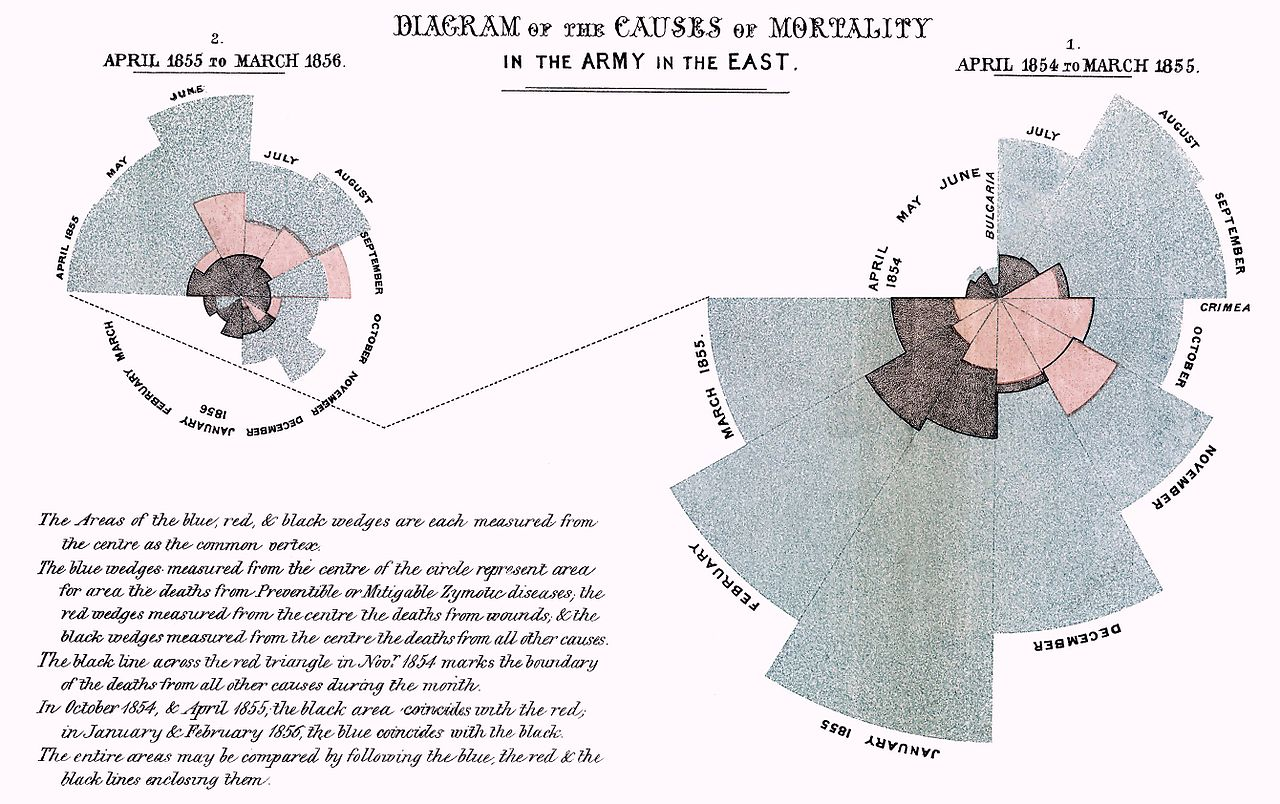
\includegraphics[width=0.8\columnwidth]{Nightingale_mortality.jpg}
   \caption{上图是南丁格尔玫瑰图。两幅图分别表示1854年和1855年军队的伤
     亡人数,
     一年12个月在极坐标上被分为12等分,每一个花瓣表示一个月;不同颜色表示死亡原因\\
     南丁格尔通过这幅图使英国政府意识到真正影响战争伤亡的并非战争本身,
     而是由于军队缺乏有效的医疗护理。由此,英国政府于1857年开设了专门的
     军医学校,培养专门的战地医护人员,\emphText{这就是统计图形在近代护
       理学最早的应用}}
 \end{figure}
\end{frame}

\subsubsection{霍乱传播之谜}
\begin{frame}{\subsecname}{\subsubsecname}
  \begin{figure}
    \begin{columns}
      \begin{column}{.6\textwidth}
        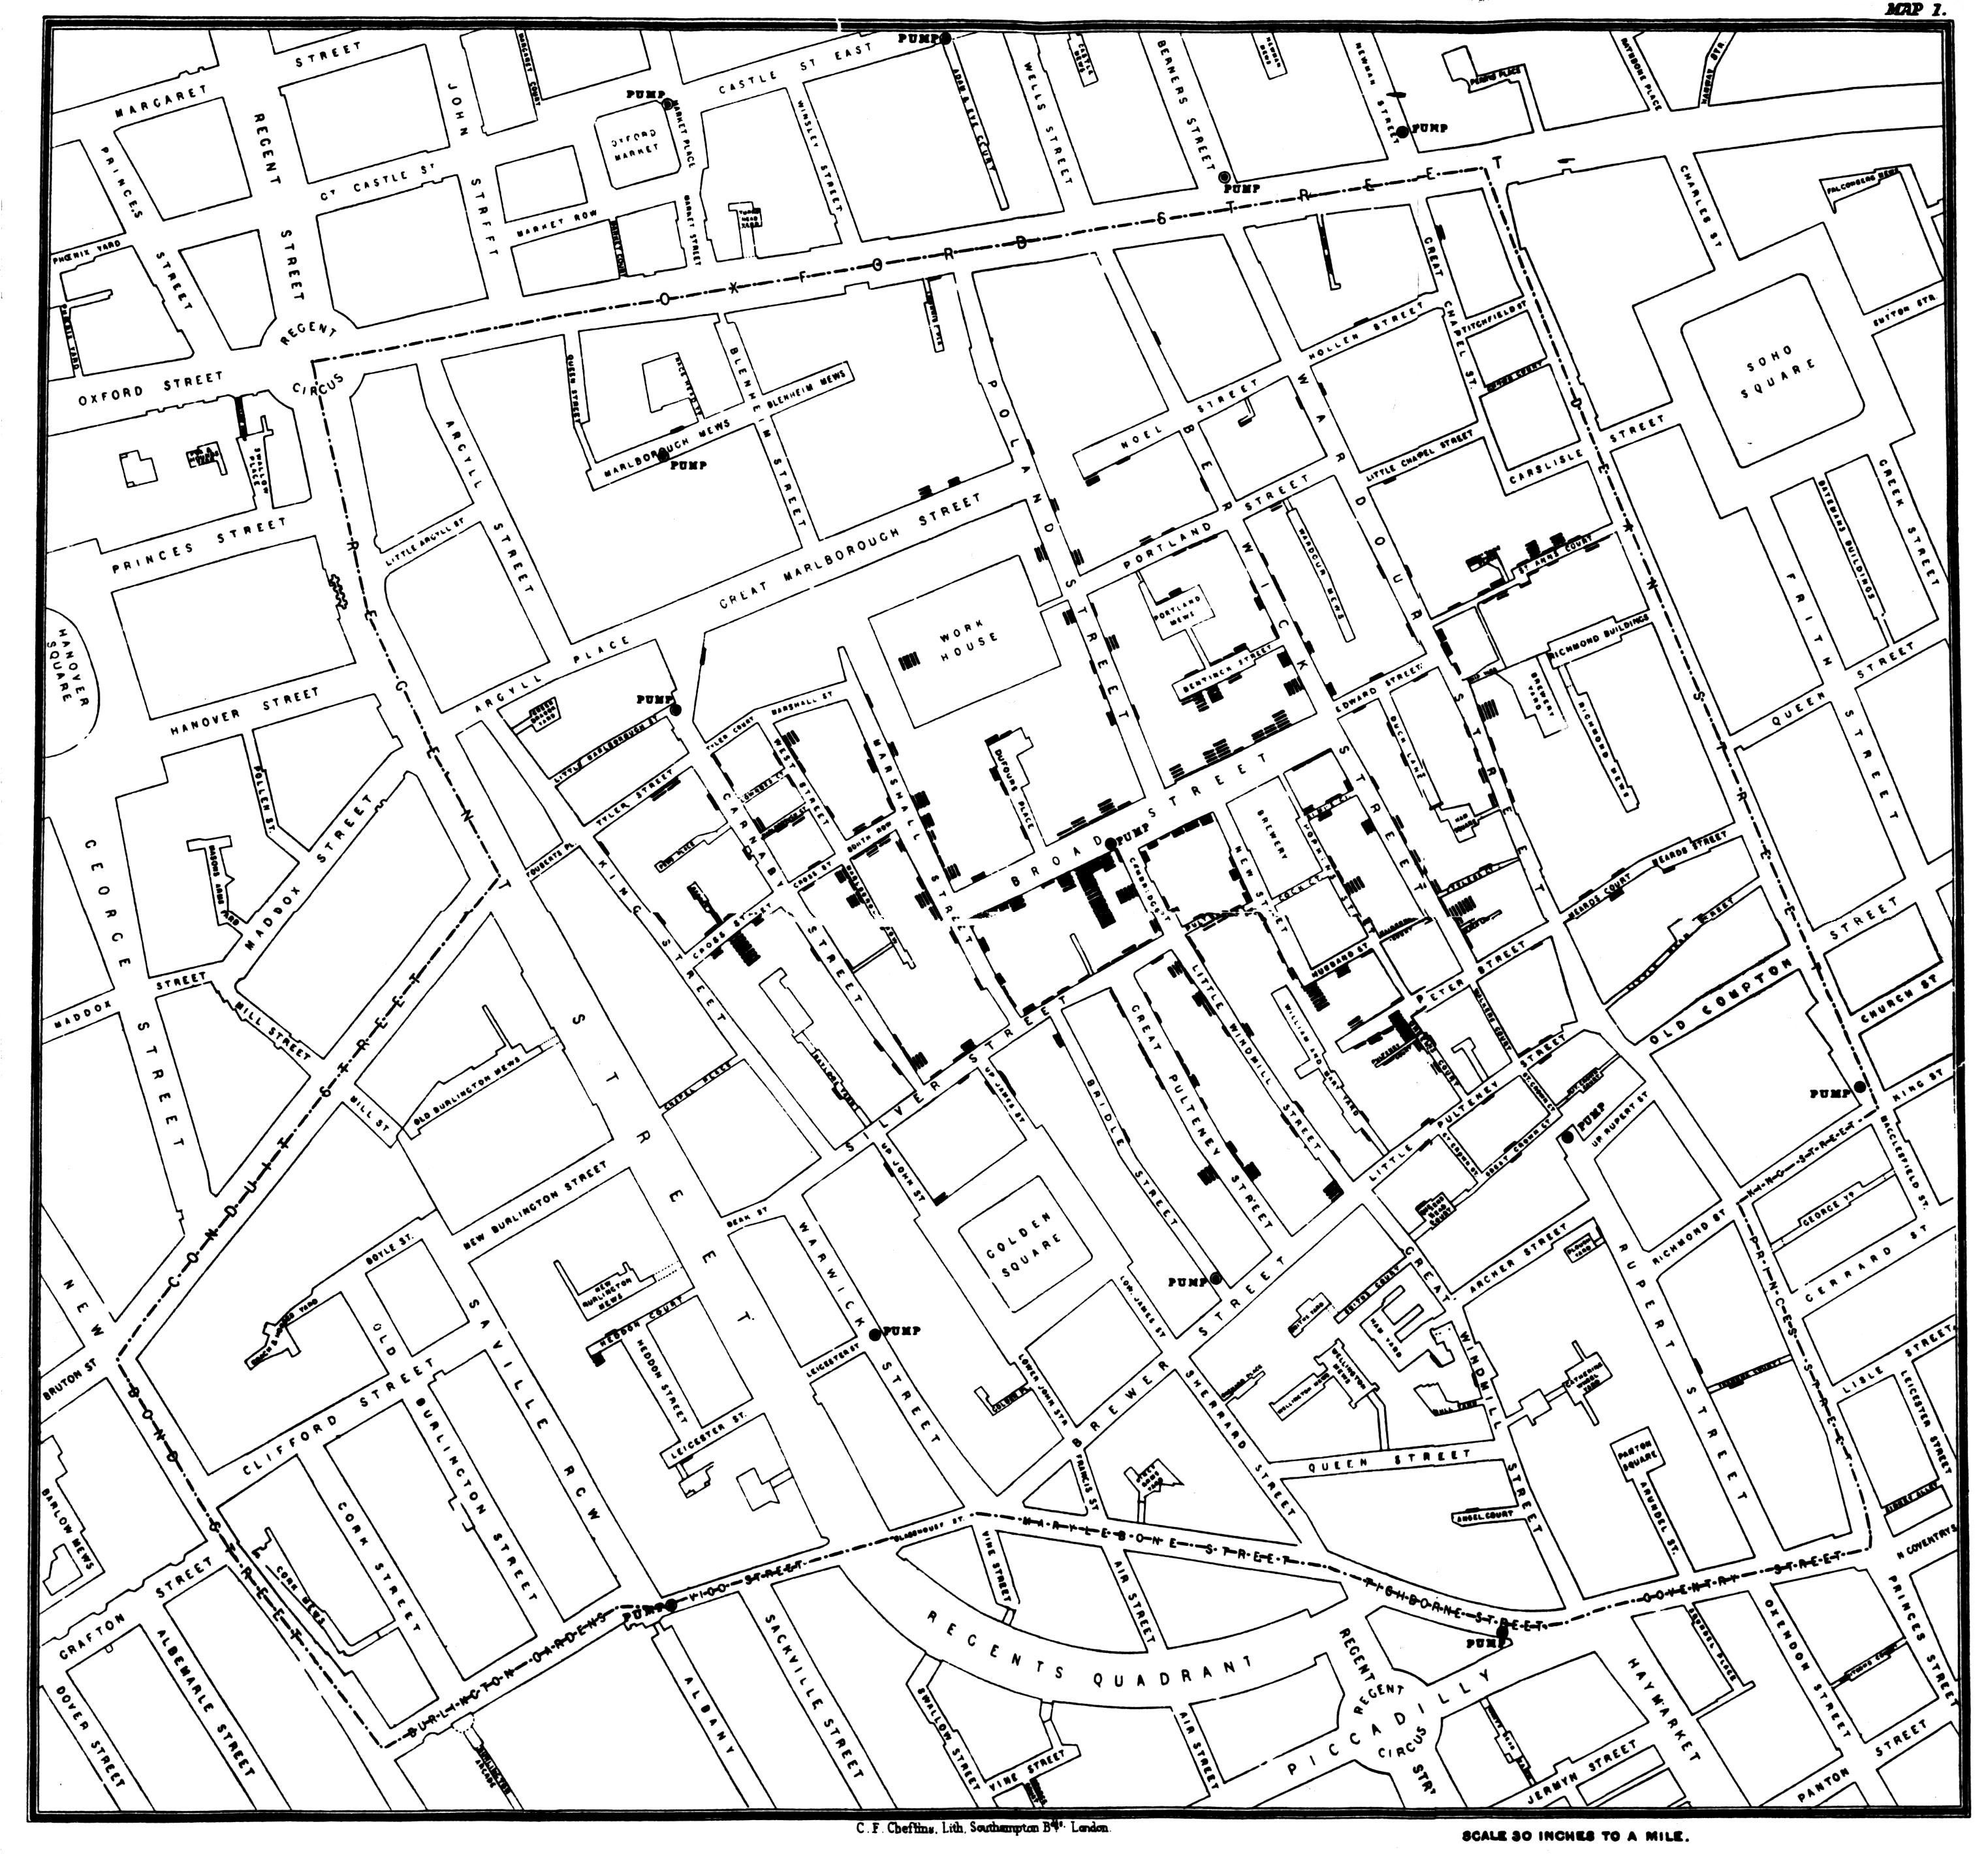
\includegraphics[width=\columnwidth]{Snow_cholera_map.jpg}
      \end{column}

      \begin{column}{.35\textwidth}
        \centering
        \caption{1854年英国Broad大街大规模爆发霍乱,流行病学家John
          Snow对此次霍乱进行了大量调研分析,并且发表了霍乱传播理论的论
          文,左图是其论文的主要依据:图中心东西
          方向的街道是Broad大街,黑点表示死亡地点\\
          这幅图形象揭示了一个重要现象,就是死亡地点都在街道中部一处水源
          (水井)周围,而市内其它水源周围极少发现死者,通过进一步调查他
          发现这些死者都饮用过这里的井水,从而发现了霍乱传播的源头是水
          井的把手,\emphText{这就是统计图形在公共卫生领域最早的应用}}
      \end{column}
    \end{columns}
  \end{figure}
\end{frame}

\begin{frame}{\subsecname}{\subsubsecname}
  \begin{figure}
    \begin{columns}
      \begin{column}{.6\textwidth}
        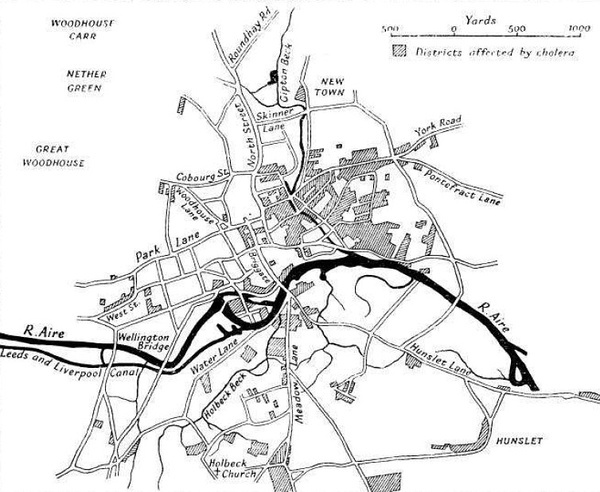
\includegraphics[width=\columnwidth]{Robert_Baker.jpg}
      \end{column}

      \begin{column}{.35\textwidth}
        \centering
        \caption{其实,在John Snow之前,有个叫Robert Baker的医生也研究
          了这个区域的霍乱问题,而且在1833年就绘制了左边这
          张霍乱的分布图。\\
          虽然Baker在这幅图中揭示了疾病和居住环境的联系:缺乏清洁用水和
          排水系统的居民点是疾病的高发区,\emphText{但是并没有显示发病
            率}。关于疾病起因的认知,他尽管方向正确但是并不完备,最终与
          伟大
          的发现擦肩而过\\
          \emphText{因此,只有充分完备的统计图形才能够真正应用于实践,
            这是一个漫长的科学过程}}
      \end{column}
    \end{columns}
  \end{figure}
\end{frame}

\subsubsection{切尔诺夫脸谱图}
\begin{frame}{\subsecname}{切尔诺夫脸谱图(Chernoff Faces)}
  \begin{figure}
    \begin{columns}
      \begin{column}{.6\textwidth}
        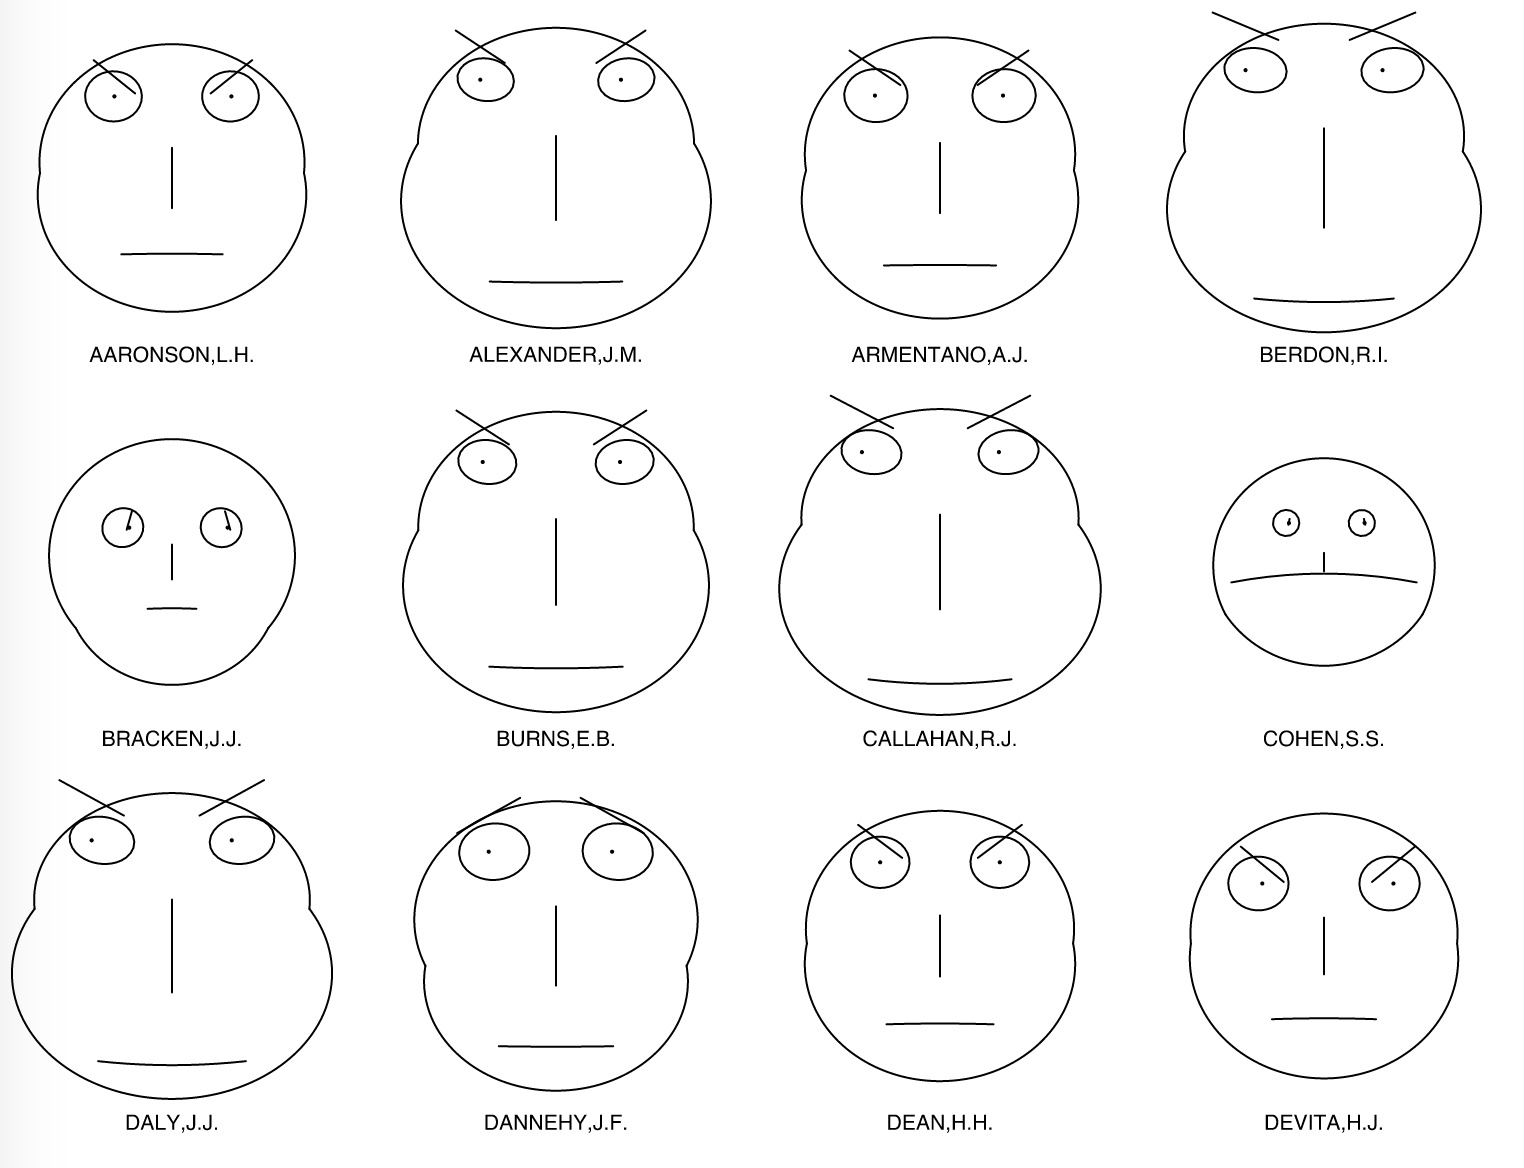
\includegraphics[width=\columnwidth]{切尔诺夫脸谱图.jpg}
      \end{column}

      \begin{column}{.35\textwidth}
        \centering
        \caption{切尔诺夫脸谱图(Herman Chernoff, 1973)\\
          这张很喜感的脸谱图其实是一种统计图,叫切尔诺夫脸谱图,是统计
          学家Herman Chernoff于1973年发明的,其基本思想是把多维数据的特
          征映射到卡通人脸中。由于人类非常善于识别脸部特征,脸谱化使得
          多维度数据容易被分析人员消化理解,有助于数据的规律和不规律性
          的可视化。\emphText{目前这种方法已被广泛应用于多地域经济战略
            指标数据分析,空间数据可视化等领域}}
      \end{column}
    \end{columns}
  \end{figure}
\end{frame}
